
\chapter{Artifact Evaluation and Discussion}

In this chapter we will evaluate the artifact from three perspectives:

\begin{enumerate}
    \item Basic web performance metrics;
    \item A systematic collection and analysis of the data produced by the artifact;
    \item Interviews with stakeholders;
\end{enumerate}


\section{Web Performance Metrics}

Using a website speed tester, we can gather useful information about the performance of the artifact, in terms of loading latency. For this test, Pingdom\footnotemark[1] was used.

\footnotetext[1]{https://tools.pingdom.com/}

Three tests were carried out, one for each of the page types:

\begin{enumerate}
    \item The about page;
    \item The artifacts browsing page;
    \item The artifact detail page;
\end{enumerate}

All tests were carried out from Pingdom's North America - USA - Washington DC location.

\subsection{About Page}


\begin{table}[H]
\footnotesize
\centering
\begin{tabular}{|ll|}
\hline
\multicolumn{1}{|l|}{\textbf{Page}} & \textbf{URL}                                                 \\ \hline
\multicolumn{1}{|l|}{About}         & http://arkivo.art/ \\ \hline
\multicolumn{2}{|l|}{\textbf{Full Test}}                                                                    \\ \hline
\multicolumn{2}{|l|}{https://tools.pingdom.com/\#64600c6e88c00000}                                 \\ \hline
\end{tabular}
\caption{Artifacts Browsing - Web Performance Test Details}
\label{table:browsing-test-details}
\end{table}


\begin{figure}[H]
    \centering
    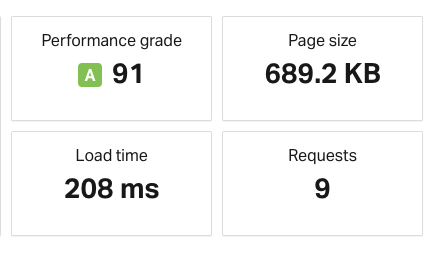
\includegraphics[width=0.5\linewidth]{about-01-general.png}
    \caption[Performance Metric: About Page (Overall)]{Performance Metric: About Page (Overall)}
    \label{fig:about-01-general}
\end{figure}

\begin{figure}[H]
    \centering
    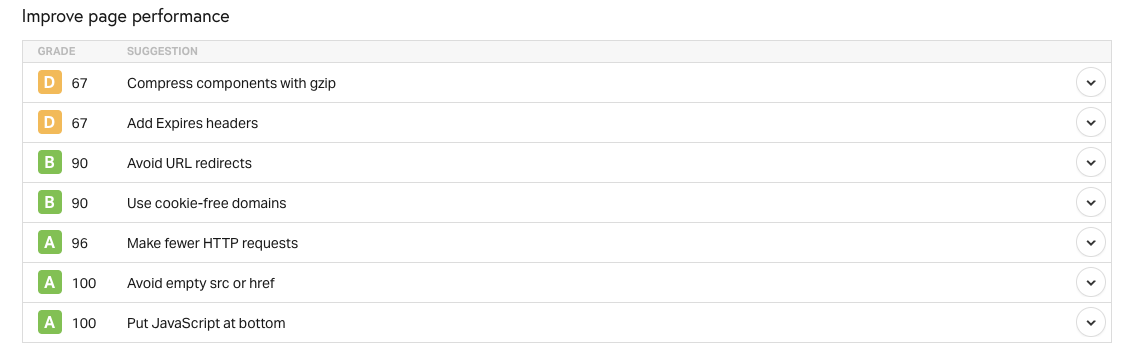
\includegraphics[width=\linewidth]{about-02-perf.png}
    \caption[Performance Metric: About Page (Improvement Areas)]{Performance Metric: About Page (Improvement Areas)}
    \label{fig:about-02-perf.png}
\end{figure}

\begin{figure}[H]
    \centering
    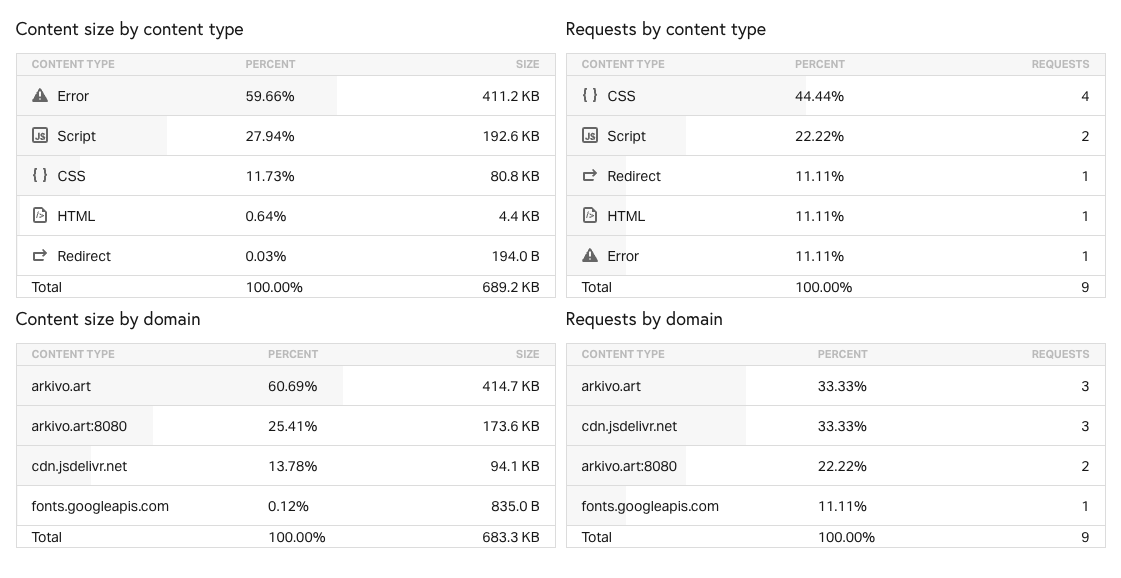
\includegraphics[width=\linewidth]{about-03-stats.png}
    \caption[Performance Metric: About Page (Content Breakdown)]{Performance Metric: About Page (Content Breakdown)}
    \label{fig:about-03-stats.png}
\end{figure}

\begin{figure}[H]
    \centering
    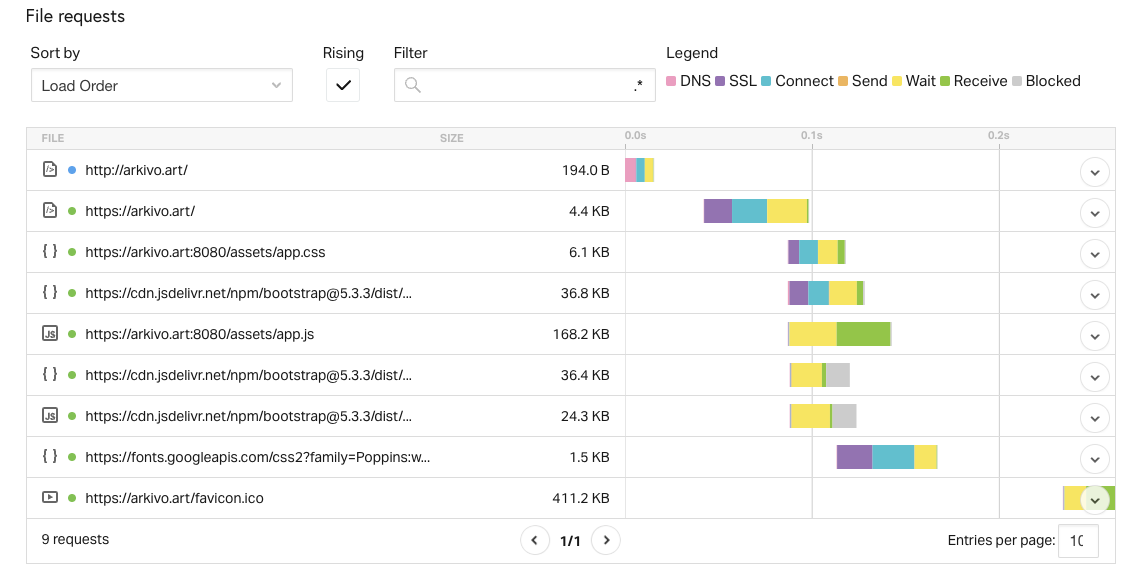
\includegraphics[width=\linewidth]{about-04-latency.png}
    \caption[Performance Metric: About Page (Loading Timeline)]{Performance Metric: About Page (Loading Timeline)}
    \label{fig:about-04-latency.png}
\end{figure}


\subsection{Artifacts Browsing Page}


\begin{table}[H]
\footnotesize
\centering
\begin{tabular}{|ll|}
\hline
\multicolumn{1}{|l|}{\textbf{Page}} & \textbf{URL}                                                 \\ \hline
\multicolumn{1}{|l|}{Artifacts Browsing}         & \multicolumn{1}{r|}{http://arkivo.art/artifacts} \\ \hline
\multicolumn{2}{|l|}{\textbf{Full Test}}                                                                    \\ \hline
\multicolumn{2}{|l|}{https://tools.pingdom.com/\#64600d6d24000000}                                 \\ \hline
\end{tabular}
\caption{Artifacts Browsing - Web Performance Test Details}
\label{table:browsing-test-details}
\end{table}


\begin{figure}[H]
    \centering
    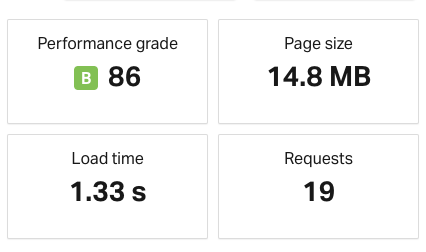
\includegraphics[width=0.5\linewidth]{artifacts-01-general.png}
    \caption[Performance Metric: Artifacts Browsing Page (Overall)]{Performance Metric: Artifacts Browsing Page (Overall)}
    \label{fig:artifacts-01-general}
\end{figure}

\begin{figure}[H]
    \centering
    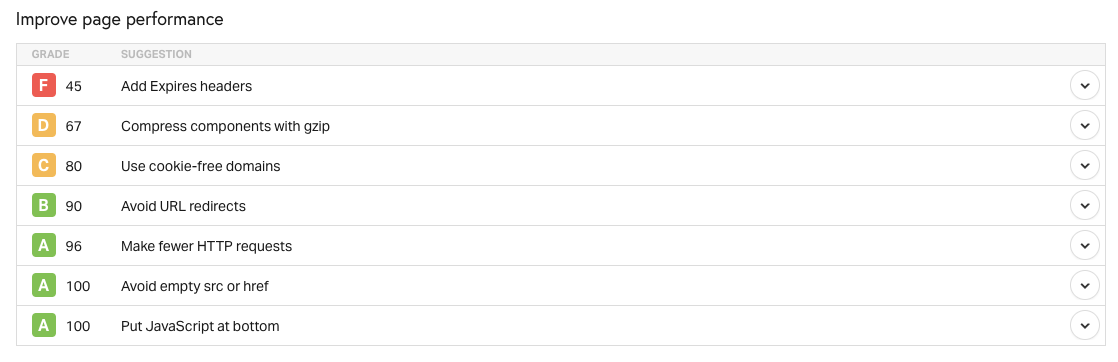
\includegraphics[width=\linewidth]{artifacts-02-perf.png}
    \caption[Performance Metric: Artifacts Browsing Page (Improvement Areas)]{Performance Metric: Artifacts Browsing Page (Improvement Areas)}
    \label{fig:artifacts-02-perf.png}
\end{figure}

\begin{figure}[H]
    \centering
    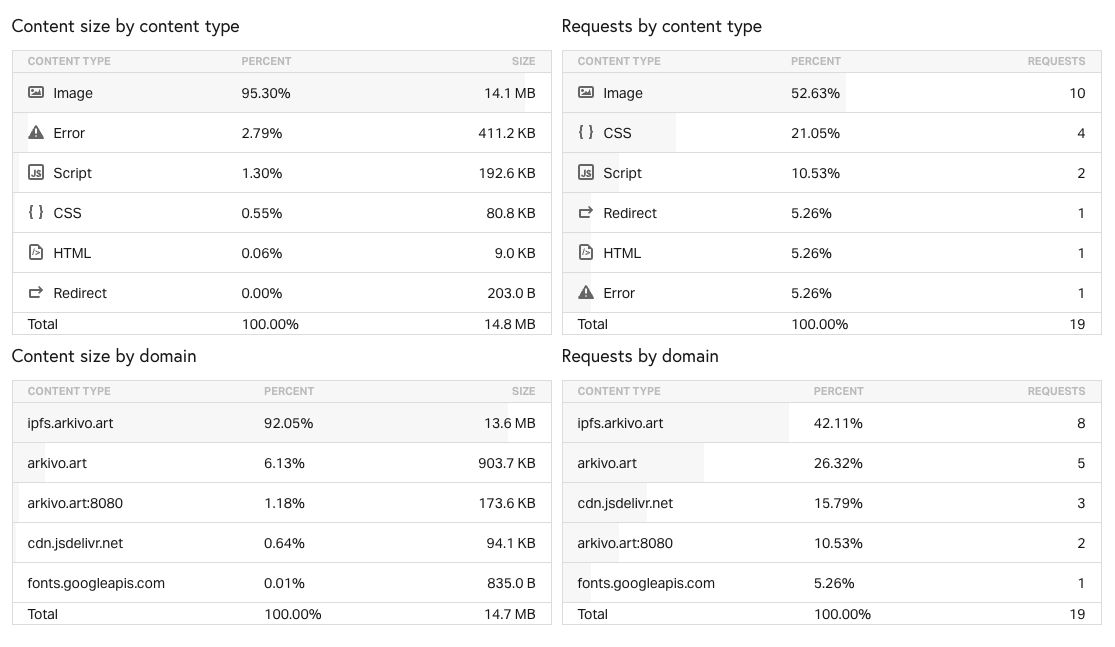
\includegraphics[width=\linewidth]{artifacts-03-stats.png}
    \caption[Performance Metric: Artifacts Browsing Page (Content Breakdown)]{Performance Metric: Artifacts Browsing Page (Content Breakdown)}
    \label{fig:artifacts-03-stats.png}
\end{figure}

\begin{figure}[H]
    \centering
    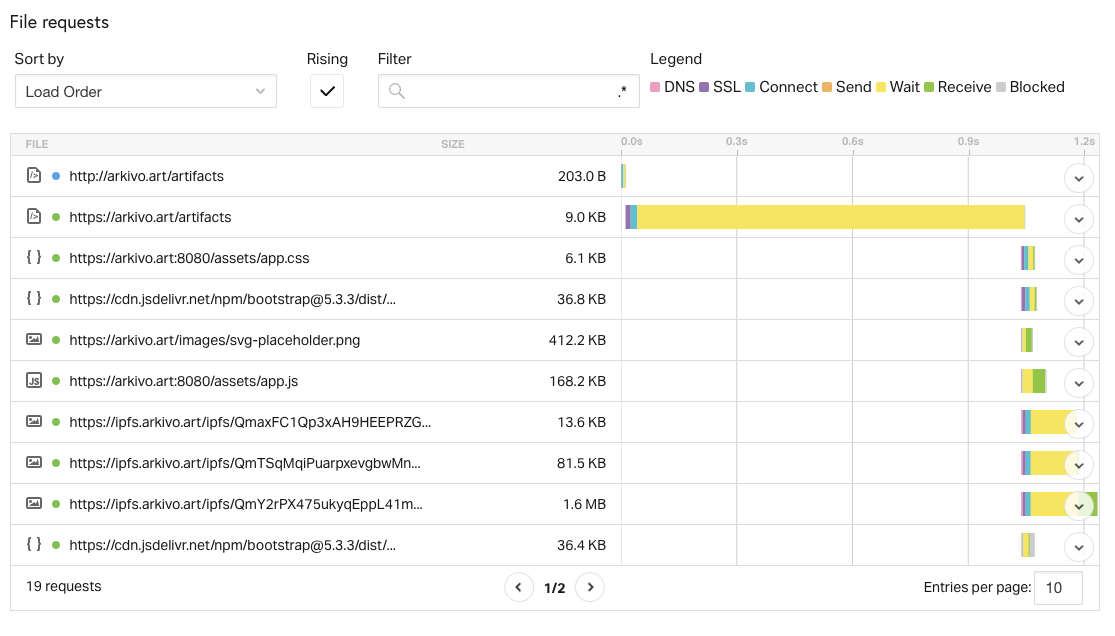
\includegraphics[width=\linewidth]{artifacts-04-latency1.png}
    \caption[Performance Metric: Artifacts Browsing Page (Loading Timeline) 1/2]{Performance Metric: Artifacts Browsing Page (Loading Timeline) 1/2}
    \label{fig:artifacts-04-latency.png}
\end{figure}

\begin{figure}[H]
    \centering
    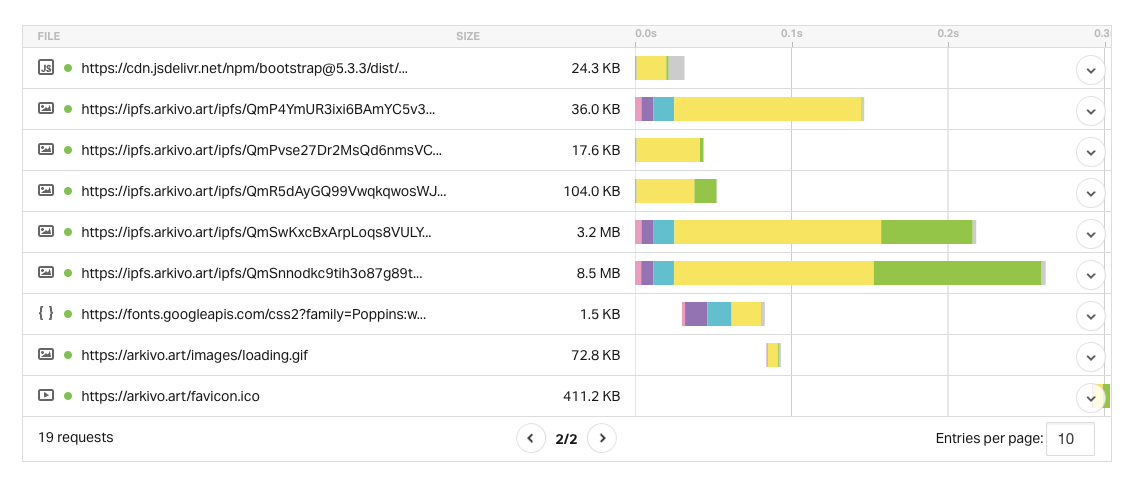
\includegraphics[width=\linewidth]{artifacts-04-latency2.png}
    \caption[Performance Metric: Artifacts Browsing Page (Loading Timeline) 2/2]{Performance Metric: Artifacts Browsing Page (Loading Timeline) 2/2}
    \label{fig:artifacts-04-latency.png}
\end{figure}


\subsection{Artifact Detail Page}

\begin{table}[h]
\footnotesize
\centering
\begin{tabular}{|ll|}
\hline
\multicolumn{1}{|l|}{\textbf{Page}} & \textbf{URL}                                                 \\ \hline
\multicolumn{1}{|l|}{Artifact Detail}         & \multicolumn{1}{r|}{https://arkivo.art/artifacts/HEN/653867} \\ \hline
\multicolumn{2}{|l|}{\textbf{Full Test}}                                                                    \\ \hline
\multicolumn{2}{|l|}{https://tools.pingdom.com/\#64600ebfd5000000}                                 \\ \hline
\end{tabular}
\caption{Artifact Detail - Web Performance Test Details}
\label{table:artifact-test-details}
\end{table}

\begin{figure}[H]
    \centering
    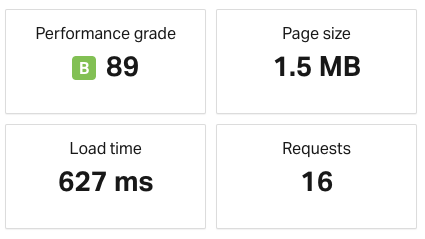
\includegraphics[width=0.5\linewidth]{artifact-01-general.png}
    \caption[Performance Metric: Artifact Detail Page (Overall)]{Performance Metric: Artifact Detail Page (Overall)}
    \label{fig:artifact-01-general}
\end{figure}

\begin{figure}[H]
    \centering
    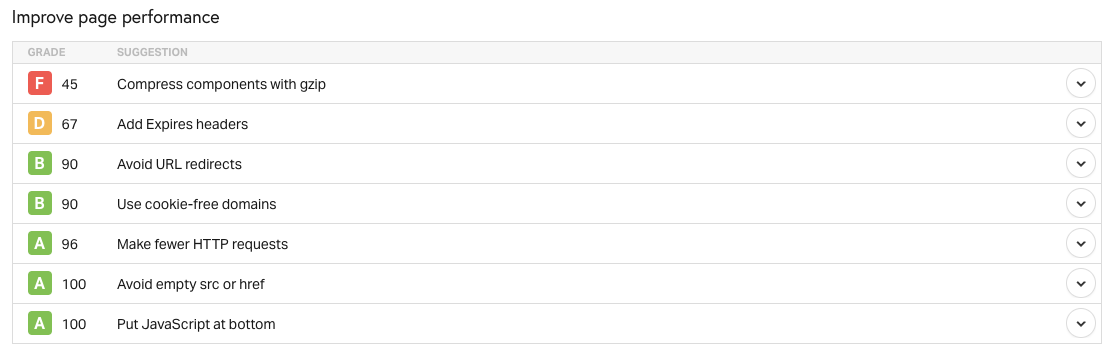
\includegraphics[width=\linewidth]{artifact-02-perf.png}
    \caption[Performance Metric: Artifact Detail Page (Improvement Areas)]{Performance Metric: Artifact Detail Page (Improvement Areas)}
    \label{fig:artifact-02-perf.png}
\end{figure}

\begin{figure}[H]
    \centering
    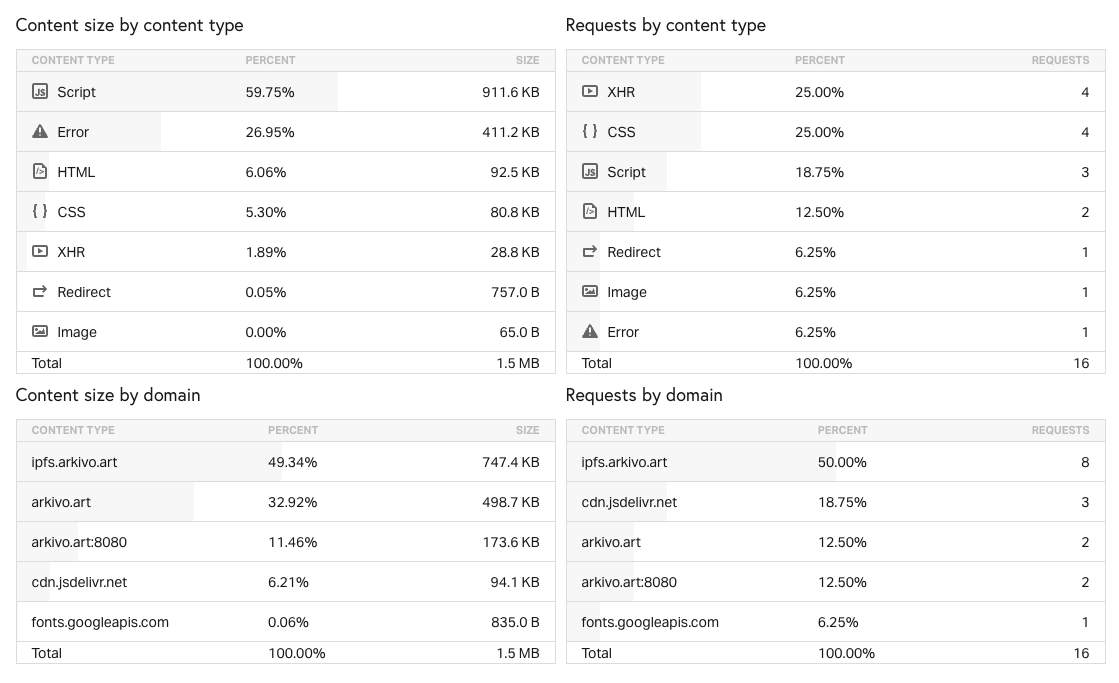
\includegraphics[width=\linewidth]{artifact-03-stats.png}
    \caption[Performance Metric: Artifact Detail Page (Content Breakdown)]{Performance Metric: Artifact Detail Page (Content Breakdown)}
    \label{fig:artifact-03-stats.png}
\end{figure}

\begin{figure}[H]
    \centering
    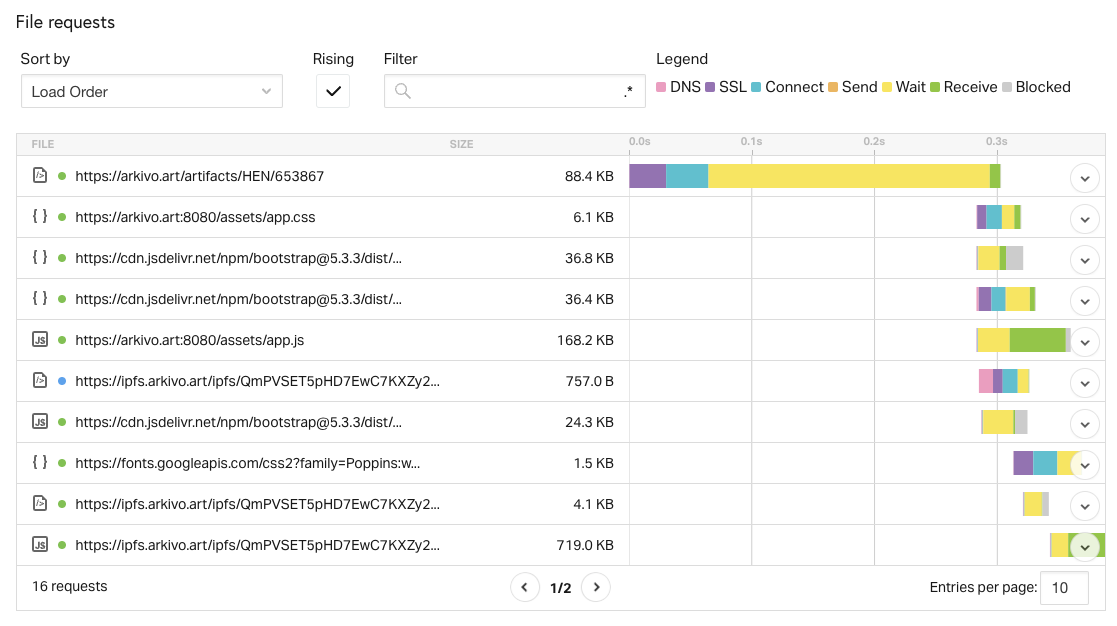
\includegraphics[width=\linewidth]{artifact-04-latency.png}
    \caption[Performance Metric: Artifact Detail Page (Loading Timeline)]{Performance Metric: Artifact Detail Page (Loading Timeline)}
    \label{fig:artifact-04-latency.png}
\end{figure}


\subsection{Web Performance Analysis}

The overall performance in terms of latency is good, although there is room for improvement. The initial page load still spends a significant amount of time in the \texttt{wait} stage, expire headers are needed, and gzip compression should also be added. Having said that, the assets loaded from the IPFS node performed better than expected.




\section{Data Analysis}

boilerplate text, boilerplate text, boilerplate text, boilerplate text, boilerplate text, boilerplate text, boilerplate text, boilerplate text, boilerplate text, boilerplate text.

\subsection{End-user study}


The 'Networked Only' checkbox caused some confusion, as one user assumed it was a filter which should instantly be reflected on the results as one checks or unchecks it. Although not originally intended as an auto-updating filter (actual filters were not implemented) the behaviour of the checkbox was altered, by adding an \texttt{onchange} event which submits the form every time it is checked or unchecked. This results in an experience that is more aligned with the user's expectations, and is a reasonable compromise until a proper filtering system is put in place.




\section{Discussion}


boilerplate text, boilerplate text, boilerplate text, boilerplate text, boilerplate text, boilerplate text, boilerplate text, boilerplate text, boilerplate text, boilerplate text.


\subsection{Capturing Interactive Artworks}
\label{subsec:capture-interactive}

One of the challenges of automating the aesthetic capture of user-interactive artworks is determining the ways in which they can be interacted with. As discussed in \autoref{sec:interactivity}, interactions can take many forms. However a manual non-exhaustive sampling of OBJKTs indexed by \texttt{ARKIVO} suggests that mouse and keyboard interactions are the most common forms of interaction in this dataset. Tools like PlayWright can simulate mouse and keyboard input during the snapshotting process, so in theory it should be possible to capture this kind of interaction. However the biggest challenge in achieving automatic interaction without any prior knowledge of the artwork is determining where in the screen to click or which keys to press. Also depending on the nature of the artwork, the interactions could be quite complex.

However a very basic experiment was attempted, using ChatGPT, to determine if a piece is interactive, and if so, where in the screen to click. As an example, the ``Jumpy Dot'' artwork by mrdoob was used.

After uploading the screenshot, the following prompts, designed to be generic and applicable to all artworks indexed by \texttt{ARKIVO}, were used:

\begin{enumerate}
	\item examine this image, and tell me if you think this represents an interactive interface
	\item if I were to click on the image to interact with it, give me approximate x,y coordinates where I should click
\end{enumerate}


The full ChatGPT chat with prompts and responses can be found in Appendix 3, page \pageref{chap:chatgpt-mouse}.

ChatGPT successfully identified the 'start' button and thus correctly classified the artwork as interactive. It also provided the following \texttt{X,Y} coordinates for click it: \texttt{255, 350}

As can be seen in \autoref{fig:chat-gpt-click-guess}, the coordinate provided by ChatGPT was relatively close, but failed to hit the 'start' button.

\begin{figure}[H]
  \centering
  \begin{subfigure}[b]{0.45\textwidth}
    \centering
    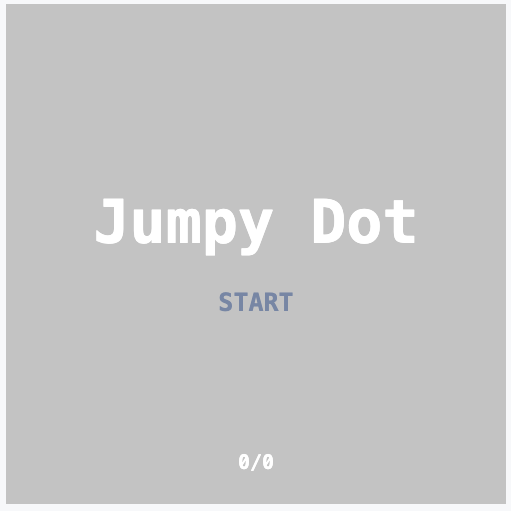
\includegraphics[width=\textwidth]{jumpydot.png}
    \caption{Input screenshot}
    \label{fig:image1}
  \end{subfigure}
  \hfill
  \begin{subfigure}[b]{0.45\textwidth}
    \centering
    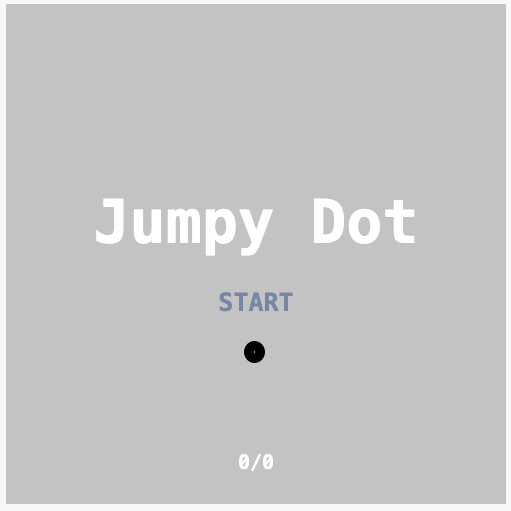
\includegraphics[width=\textwidth]{jumpydot-click.png}
    \caption{ChatGPT coordinate guess}
    \label{fig:image2}
  \end{subfigure}
  \caption{ChatGPT estimated interaction coordinate}
  \label{fig:chat-gpt-click-guess}
\end{figure}

It should be noted that this artwork, due to the simplicity its the interface, and the explicit nature of the 'start' button, constitutes one of the easiest possible tests for an LLM like ChatGPT to determine interactivity and hotspot locations for interactions. The fact that it failed to provide the correct coordinate suggests there is still a gap between the textual description of the location of the button, "close to the center horizontally [...] slightly below the center vertically" and the prediction of the coordinate.

The LLM approach to UI interaction is fairly new, but some research is starting emerge \cite{liuMakeLLMTesting2024}, and more is expected to follow.

Alternative strategies for interacting with the artwork can also be experimented with. For example, the Android development ecosystem has a tool, UI/Application Exerciser Monkey, which generates pseudo-random streams of user events such as clicks, touches, or gestures for automated UI testing \cite{UIApplicationExerciser}.

\subsection{Cost of Storage}

Currently, the cost of minting an OBJKT on the HEN contract constitutes a fraction of the cost of hosting and/or pinning 2GB of data. This represents a loophole that could be exploited by malicious actors, or freeloaders, making the pinning of assets hosted by Teia unfeasible without a significant recurring investment, which impacts the economic sustainability of the project.

\subsection{Emulation}

As time passes, technology will continue to evolve. New hardware will run new operating systems, which will run new web browsers, or even totally paradigm changing \emph{content rendering applications} which may replace web browsers in the future. This means that in long term it seems inevitable that all code-base artworks created today, even those based on web standards and without any network dependencies, will require some form of hardware and/or browser emulation to render successfully. 

This inevitable evolution into emulated environments does represent an additional challenge for networked artworks, because in addition to emulating the artefact's code-base itself, the emulation environment must also simulate the network dependencies of the artwork, and this can pose a problem known to software developers as \emph{dependency hell}, where each dependency in turn depends on a number of other dependencies, leading to an ever increasing dependency tree. A solution to this problem seems unfeasible, if any of those dependencies, or their sub-dependencies, does not strictly follow the web3 architecture that makes projects easily duplicable.

For this reason, the IOC model gains an even greater importance for the longevity of code-based networked artworks, because you can more easily generate the data expected by the artwork, or in the worst-case scenario, simply repeatedly inject the last known good snapshot of data for all future renderings.

\subsection{Beyond the Canvas}

All of the artworks which this project currently aims to cater for in terms of conservation have one thing in common: their visual rendering is restricted to the boundaries of an HTML element on a web page, the canvas. Even those which intentionally choose to spread their visual expression past the boundaries of a single canvas element, are still constrained by the larger HTML DOM object or web page in which they, as web-based artworks, essentially exist. This is not unique to digital art. The great majority of paintings displayed in traditional museums are also constrained by their physical framed canvasses. Sculptures and other art installations are exceptions to this rule. However networked art reaches out into the world, and it would seem appropriate to explore a rendering medium that represents that breaking away from the canvas.


\subsection{Identifying IPFS Pinning Abuse}

Since most IPFS pinning services are paid for, there is a potential for abuse of free pinning services like Teia, and now Arkivo, by mining directory-x OBJKTs just as a way to store data on IPFS for free. The OBJKT might even render a piece of original art, but just as a facade for a much larger data payload. This would add to an archive's storage costs without contributing back in terms of donation, hurting its sustainability.


On the other hand, if the art has value, 

